\chapter{集合与简易逻辑}

 \section{集合}
\subsection{集合的概念}
我们在第一册中曾用到过集合的概念,如自然数所构成
的集合$\{1,2,3,\ldots\}$, 方程$x^2=4$的解所构成的集合$\{-2,2\}$
等等。那么,什么是集合呢?集合是数学中一个很根本的也
是很原始的概念,通常我们把一些确定的、彼此不同的“事
物”作为一个整体来考虑时,这个整体便说是一个\textbf{集合}。这
些事物叫做该集合的\textbf{元素}。例如:
某中学初二(一)班全体学生;小于100的全体质数;
一个生产队的全体社员;一个工厂的全部机器等等,都可分别构成一个集合。可见集合的概念是很简单
的。

对于集合这个概念,我们要注意以下几点:

第一,一个集合完全被它所含的元素所确定。至于集合
的元素之间是否具有某种相互关系,怎样排列,以及这些元
素所构成的集合是具有某种功效,单从集合的观点来看,
是一样的。例如,“一堆还没有组装的手表另件”和用“这
些另件组装好了的手表”是同一个集合。因为两者包含同样
的元素。因此,集合这个概念的要素是:\textbf{一个集合完全被它
所含的元素所确定}。

第二,集合是指构成集合的全体元素,而不是个别元
素。作为整体的集合和集合中的每个元素都是不同的。

例如,集合$A=\{a,b,c,d\}$, $A$代表的是字母$a$、$b$、
$c$、$d$的全体,而不是代表其中的个别字母,因此,作为字母
$a$、$b$、
$c$、$d$的整体的集合$A$与$A$中的个别元素如$a,b,c,d$不
能混为一谈。

第三,集合中所含的元素必须是“确定”的,是可以判
断的。例如,由“比较小的实数”的全体就不能构成一个集
合,因为到底什么叫做比较小的实数,没有判断的标准。但
是“比80小的实数”是完全可以确定的,这就有了检验一个
实数是否是这个集合的元素的标准。

任一几何图形,我们可以看作由点构成的,也就是可看
作点的集合。例如:

\textbf{圆}是同一平面上与一定点的距离等于定长的所有点的集
合(图2.1(1))。

\textbf{圆面}是同一平面上与一定点距离小于或等于定长的所有
点的集合。(图2.1(2))。

\begin{figure}[htp]
	\centering
	\begin{tikzpicture}[scale=.7]
		\begin{scope}
			\draw (0,0) circle (2);
\draw[ultra thick] (0,0)node[below]{$O$}--node[left]{$r$}(45:2);		
\node at (0,-3){(1)圆};	
		\end{scope}
		\begin{scope}[xshift=6cm]
			\draw[pattern=north west lines] (0,0) circle (2);
\draw[ultra thick] (0,0)node[below, fill=white]{$O$}--(45:2);	
			\node at (60:1.5) [left, rotate=45, fill=white]{$r$};
			
			\node at (0,-3){(2)圆面};
		\end{scope}
	\end{tikzpicture}	
	\caption{}
\end{figure}

我们通常用大写字母$A,B,C,\ldots$等表示某一个集合,
用小写字母$a,b,c,\ldots$表示集合的元素。如果$a$是集合$A$
的一个元素,我们就记为$a\in A$,
读作$a$属于$A$, 或说$a$是$A$中的一个元素。例如,$2\in\{2,3\}$,
表示$2$是集合$\{2,3\}$中的一个元素。

如果$a$不是集合$A$的元素,记作
$a\notin A$
读作$a$不属于$A$。

应该注意的是:几何图形中的元素“点”我们仍用大写
字母$A,B,C,\ldots$表示,这一点
请同学们务必注意,不要混
淆。如$X$点在直线$AB$上,也
可以说$X$点属于直线$AB$, 可
写成$X\in\text{直线}AB$. $Y$点不在直
线$AB$上,也可以说$Y$点不属于直线$AB$, 可写成$Y\notin\text{直线}
AB$(图2.2)。

\begin{figure}[htp]
	\centering
	\begin{tikzpicture}[scale=1]
\draw(0,0)--(6,0);
\draw (1,0)[fill=black]circle (1.5pt) node[below]{$A$};
\draw  (4.5,0)[fill=black]circle (1.5pt) node[below]{$B$};
\draw  (4,-.5)[fill=black]circle (1.5pt) node[below]{$Y$};
\draw  (3,0)[fill=black]circle (1.5pt) node[above]{$X$};
	\end{tikzpicture}	
	\caption{}
\end{figure}

\begin{ex}
\begin{enumerate}
\item 若$S$是
所有平方数的集合,试判定100至200之间哪些数
属于$S$.
\item 若$B$是所有英语元音字母所构成的集合,$A$是所有英语
辅音字母所构成的集合,试判定$a,b,c,d,e$这五个字
母分别属于哪一集合,又不属于哪一集合。
\end{enumerate}
\end{ex}

\subsection{集合的描述法}
决定一个集合的要素,就是它所含的元素,所以要描述
一个集合,也就是要描述它所含的是哪些元素。下面介绍两
种常用的集合描述法。

\subsubsection{列举法}
如果一个集合$A$只含有很少几个元素,那么可以直截了
当地把这个集合含有的所有元素逐一列举出来,并用大括号
$\{\quad \}$把它们括起来,这种描述法叫做\textbf{列举法}。

例如$\{0,1\}$是由0,1这两个元素所构成的集合;$\{+,-,\x,\div\}$表示由$+$、$-$、$\x$、$\div$四个运算符号所构成的
集合。用列举法描述集合时,描述方法与元素在括号内的排
列顺序无关,即$\{3,7,10\}$、$\{10,3,7\}$与$\{7,3,10\}$
都表示同一个集合。

\subsubsection{特征性质描述法}
当集合的元素稍多一些时,如小于100的质数所构成的
集合:$$\{2,3,5,7,11,13,17,19,23,29,31,37,
41,43,47,53,59,61,67,71,73,79,83,89,
97\}$$
逐一列举已是很麻烦的了,而对于含有无穷多个元素的
集合,例如全体整数所构成的集合,逐一列举它的元素更是
不可能的,这时我们可用某集合所含的元素的“特征性质”
去描述这个集合,这种方法叫做\textbf{特征性质描述法}。如:

\begin{enumerate}
\item 集合元素为
$\pm 2,\pm 4,\pm 6,\pm 8,\ldots,\pm 2n\ldots$的集
合,可描述为\{偶数}或\{能被2整除的数}。
\item 集合元素为$\pm 1,\pm 3,\pm 5,\pm 7,\ldots,\pm (2n+1)\ldots$的集合,可描述为\{奇数\}或\{被2除余1的数\}。
\item $\{-\sqrt{2},\sqrt{2}\}$,可描述为$\{\text{平方为2的数}\}$。
\item 圆面上不在圆上的点叫做圆内的点。在平面$P$上以$O$为
圆心,5厘米长为半径的圆内的点所成的集合,可描述为\{在
平面$P$上和点$O$的距离小于5厘米的点\}。	
\end{enumerate}

集合的特征性质描述法,常常采用下面更一般的形式:
\[A=\{x|\alpha\}\]
其中$x$表示集合$A$的任一元素,$x|\alpha$表示元素$x$具有特征性
质$\alpha$, 而$A=\{x|\alpha\}$则表示由所有具有性质$\alpha$的元素所构
成的集合$A$. 这样一来,上述各例又可表示如下:
\begin{enumerate}
    \item $A=\{x|x\text{能被2整除}\}$
    \item $B=\{x|x\text{被2除余1}\}$
    \item $C= \{x|x^2=2\}$
    \item $D=\{X|\overline{OX}<5{\rm cm},\; \text{且$O$是平面$P$上定点,$X\in$平面$P$} \}$
\end{enumerate}

有时候“任一元素$x$”也可用某种形式写出来,例如上面的集合$A$、$B$可写为:
\[\begin{split}
    A&=\{2n|n\text{为任意整数}\}=\{2n|n\in\mathbb{Z}\}\\
    B&=\{2n+1|n\text{为任意整数}\}=\{2n+1|n\in\mathbb{Z}\}
\end{split}\]

\begin{ex}
\begin{enumerate}
    \item 用列举法表示下列集合:
\begin{enumerate}
    \item 头五个质数的全体构成的集合。
    \item 12的所有因数构成的集合。
    \item 自然数里头五个平方数的全体构成的集合。
    \item 20与30间的奇数的全体构成的集合。
    \item 小于20的全体偶数构成的集合$P$。
\end{enumerate}

\item 用符号“$\in$”,“$\notin$”表示$b$, $c$, $d$与集合的关系。
\begin{enumerate}
    \item $A=\{x|x\text{是15的因数}\}$,$b=5$, $c=15$, $d=12$;
    \item $O=\{x|x\text{是小于16的质数}\}$,$b=2$, $c=3$, $d=7$。
\end{enumerate}

\item $C$是平面$P$上以$O$为圆心,半径为3cm的圆周上的所有点组
成的集合,$X$、$Y$、$Z$是平面$P$上的三个点,且$\overline{OX}=5{\rm cm}$, $\overline{OY}=2{\rm  cm}$, $\overline{OZ}=3{\rm cm}$, 试用符号“$\in$”和“$\notin$”表示$X$,
$Y$, $Z$与集合$C$的关系。

\item 试用特征性质描述法描述下列集合。
\begin{enumerate}
    \item 一元二次方程$x^2+2x-3=0$的两个根所构成的集合。
    \item 所有加7就大于15的实数所构成的集合。
    \item 所有大于或等于3而小于5的实数的集合。
\end{enumerate}

\item 试用特征性质描述第1题中的五个集合。

\item 把下列集合用列举法描述出来:
\begin{enumerate}
    \item $A=\{x|x\text{是整数且}|x|<5\}$
    \item $B=\{x|x\text{是英语中的元音字母}\}$
    \item $C=\{x|x\text{是整数且}1<x<10  \}$
    \item $D=\{x|x\text{是$a$或是$b$,或是$c$}\}$
\end{enumerate}
\end{enumerate} 
\end{ex}

\subsection{集合与集合的关系和集合的运算}

\subsubsection{集合与集合的关系}
如果集合$A$的每一个元素,也是集合$B$的元素,那么我们说$A$是$B$的\textbf{子集}。也可以说“$A$\textbf{含于}$B$”,或“$B$\textbf{包含}$A$”,我们用符号$A\subseteq B$, 或$B\supseteq A$来表示,请同学们注意:因为集合$A$的每个元素肯定是集合$A$的一个元素,所以每个集合$A$都是它本身的子集。

为了能够形象化地帮助我们理解集合,我们常用图来表示集合。最常用的方法是对给定的集合用圆形表示,圆形上的点表示该集合的元素,圆形外的点表示不是该集合的元素。不同的圆形表示不同的集合。这种圆形通常叫做维恩(Venn)图。

这样,集合$A$是集合$B$的子集,可形象地用图2.3所示的两圆形来表示。

如果集合$A$中的每一个元素都是集合$B$中的元素,而$B$中的元素却有不属于$A$的,这时我们说$A$是$B$的\textbf{真子集},记作$A\subset B$。
\begin{figure}[htp]\centering
    \begin{minipage}[t]{0.48\textwidth}
    \centering
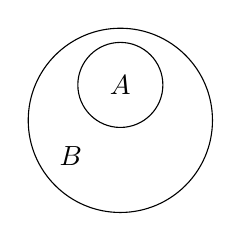
\begin{tikzpicture}[>=latex, scale=.9]
\draw (0,0) circle (.6);
\draw (0,-.5) circle (1.3);
\node at (0,0){$A$};
\node at (-.7,-1){$B$};
    \end{tikzpicture}
    \caption{}
    \end{minipage}
    \begin{minipage}[t]{0.48\textwidth}
    \centering
    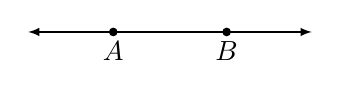
\begin{tikzpicture}[>=latex, scale=.9]
\draw[<->](-2,1)--(2,1);
\draw (-.8,1) [fill=black]circle (1.5pt)node[below]{$A$};
\draw (.8,1) [fill=black]circle (1.5pt)node[below]{$B$};
    \end{tikzpicture}
    \caption{}
    \end{minipage}
    \end{figure}

在图2.4中,$\overline{AB}$上的点都是直线$AB$上的点,但是直线$AB$上的点却还有很多不属于$\overline{AB}$, 所以$\overline{AB}$是直线$AB$的真子集,记作:
\[\overline{AB}\subset \text{直线}AB\]

这里我们要提醒同学们注意区分“属于”关系和“含于”关系。“属于”关系是集合的元素与集合本身的关系,但“含于”关系却是集合与集合之间的关系。

例如集合$A=\{3, 4, 5\},\; B=\{3, 4, 5, 6, 7\}$, 对于元素4来说,它和$A$或$B$的关系是“属于”关系,即$4\in A$, $4\in B$; 对于集合$A$与$B$来说,它们的关系却是“含于”关系,即$A\subset B$。

如果两个集合$A$、$B$是由共同的元素所构成的,我们称它们为相等的集合,记作$A=B$. 例如,$\{x,y,z\}=\{y,x, z\}$, $\{+, -, \x, \div \}=\{ \x, -,+,\div\}$等。

如果两个集合$A$、$B$, $A\subseteq B$且$B\subseteq A$, 这就是说$A$的每个元素都是$B$的元素,而$B$的每个元素也都是$A$的元素,显然这两个集合含有相同的元素,则$A=B$. 例如,$A=\{\text{偶数}\}$,$B=\{2n|n\in\mathbb{Z}\}$, 则$A=B$. 事实上$A$, $B$两个集合
就是同一个集合的两种不同描述法。

如果有三个集合$A$、$B$、$C$, $A\subseteq B$且$B\subseteq C$, 那么显然有$A\subseteq C$. 这就是说集合的含于关系具有传递性。

\subsubsection{集合的运算}

\paragraph{交集}
由集合$A$与集合$B$的公共元素所成的集合叫做集合$A$与集合$B$的交集(或交)。记为:
$A\cap B$,读为$A$交$B$.
\begin{figure}[htp]\centering
    \begin{minipage}[t]{0.48\textwidth}
    \centering
\begin{tikzpicture}[>=latex, scale=1]
    \draw (0,0)node{$A$} circle(.75);
    \draw (1.3,0)node{$B$} circle (1);
    \draw[->](.5,-1.3)node[below]{$A\cap B$}--(.5,-.7);
    \clip {(0,0) circle (.75)};
    \fill[pattern=north east lines] {(1.3,0) circle (1)};
    
    \end{tikzpicture}
    \caption{}
    \end{minipage}
    \begin{minipage}[t]{0.48\textwidth}
    \centering
    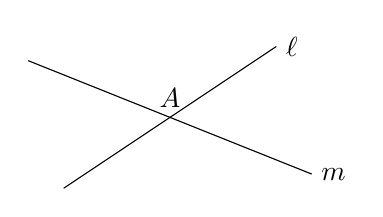
\begin{tikzpicture}[>=latex, scale=.9]
\draw (-2,.8)--(2,-.8)node[right]{$m$};
\draw (-1.5,-1)--(1.5,1)node[right]{$\ell$};
\node at (0,0)[above]{$A$};
    \end{tikzpicture}
    \caption{}
    \end{minipage}
    \end{figure}


两个集合$A$、$B$的交集用维恩图来示意,如图2.5中的阴影部分就表示$A\cap B$.

若$A=\{ a, b, c, d \}$, $B=\{ c, d, e\}$, 则$A\cap B=\{c,d\}$。

在图2.6中,直线$\ell$与直线$m$的交集是$A$点,即$\ell \cap m=\{A\text{点}\}$。
\begin{figure}[htp]\centering
    \begin{minipage}[t]{0.48\textwidth}
    \centering
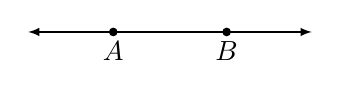
\begin{tikzpicture}[>=latex, scale=.9]
\draw[<->](-2,1)--(2,1);
\draw (-.8,1) [fill=black]circle (1.5pt)node[below]{$A$};
\draw (.8,1) [fill=black]circle (1.5pt)node[below]{$B$};
    \end{tikzpicture}
    \caption{}
    \end{minipage}
    \begin{minipage}[t]{0.48\textwidth}
    \centering
    \begin{tikzpicture}[>=latex, scale=.9]

    \end{tikzpicture}
    \caption{}
    \end{minipage}
    \end{figure}

在图2.7中,$\overline{AB}$是射线$AB$和射线$BA$的交集,即:
\[\overline{AB}=\text{射线}AB\cap \text{射线}BA\]

一条直线把一个平面分成两部分,其中每一部分都叫做半平面,这条直线叫作半平面的界。图2.8中,$\angle AOB$的内部是以直线$OA$为界含有射线$OB$的半平面与以直线$OB$为界含有射线$OA$的半平面的交集(即图中的阴影部分)。

\begin{figure}[htp]\centering
    \begin{minipage}[t]{0.48\textwidth}
    \centering
\begin{tikzpicture}[>=latex, scale=1]
\fill[draw, pattern=north east lines] (0,0)node[fill=white]{$A$} circle(.75);
\fill[draw, pattern=north east lines]  (1.3,0)node[fill=white]{$B$} circle (1);
    \end{tikzpicture}
    \caption{}
    \end{minipage}
    \begin{minipage}[t]{0.48\textwidth}
    \centering
    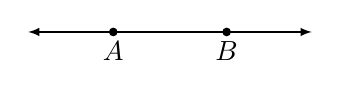
\begin{tikzpicture}[>=latex, scale=.9]
\draw[<->](-2,1)--(2,1);
\draw (-.8,1) [fill=black]circle (1.5pt)node[below]{$A$};
\draw (.8,1) [fill=black]circle (1.5pt)node[below]{$B$};
    \end{tikzpicture}
    \caption{}
    \end{minipage}
    \end{figure}

显然,若$A\subseteq B$, 则$A\cap B=A$, 反之,若$A\cap B=A$, 则$A\subseteq B$.

\paragraph{并集}
由集合$A$的元素或集合$B$的元素合并而成的
集合叫做集合$A$与集合$B$的并集(或并)记为:
$A\cup B$,读为A并B。

集合$A$与集合$B$的并集用维恩图示意,如图2.9所示,图中的阴影部分就表示$A\cup B$.

如果$A=\{1, 2, 3\}$, $B=\{3, 4, 5\}$, 那么$A\cup B= \{1, 2, 3, 4, 5\}$.

\begin{rmk}
    在求上述$A$、$B$的并集时,虽然$A$与$B$含有共同的元素3, 但在$A\cup B$中3只取一次。
\end{rmk}

如果$A_+=\{x|x\text{是实数,且}x\ge 5\}$,$A_-=\{x|x\text{是实数,且}x\le -5\}$,$A=\{x|x^2\ge 25\}$,那么$A_+\cup A_-=A$。

在图2.10中,直线$AB$是射线$AB$和射线$BA$的并集,即
\[\text{直线}AB=\text{射线}AB \cup \text{射线}BA\]

\paragraph{空集}
为了使集合$A$和集合$B$的交集$A\cap B$在集合$A$与集合$B$不含有任何公共元素时仍有意义,我们自然想到:这时的$A\cap B$应是一个不含有任何元素的集合。因此,我们把这种不含任何元素的集合叫做\textbf{空集},并用符号$\emptyset$表示。

由空集的意义可知,对任何一个集合$P$, 都有$P\cap \emptyset=\emptyset$, $P\cup\emptyset=P$成立,并且空集是任何一个集合$P$的子集。即:$P\supseteq \emptyset$

如果$A=\{\text{奇数}\}$,$B=\{\text{偶数}\}$,那么$A\cap B=\emptyset$。

在图2.11中,若$\odot O_1$和$\odot O_2$相离,则$\odot O_1\cap \odot O_2=\emptyset$
\begin{figure}[htp]
    \centering
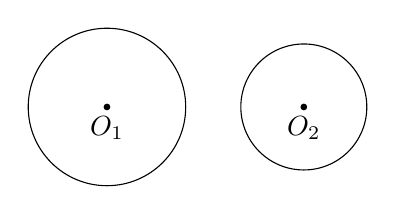
\begin{tikzpicture}
\draw (0,0)node[below]{$O_1$} circle (1);
\draw (2.5,0)node[below]{$O_2$} circle (.8);
\draw (0,0) [fill=black] circle(1pt); 
\draw (2.5,0) [fill=black] circle(1pt); 
\end{tikzpicture}
    \caption{}
\end{figure}

如果直线$a\parallel$直线$b$, 那么$a\cap b=\emptyset$.

\paragraph{基集与补集}

如果我们所讨论的集合都是一个给定集合的子集,我们就称这个给定集合为\textbf{基集},通常用符号$I$表示基集。

例如,我们所讨论的集合是$\emptyset$、$\{1\}$、$\{2\}$、$\{3\}$、$\{1, 2\}$、$\{2, 3\}$、$\{1, 3\}$和$\{1, 2, 3\}$时,因为上述集合都是集合$\{1, 2, 3\}$的子集,所以我们称$\{1, 2, 3\}$为基集。

又因为平面和平面上的几何图形都是点的集合,那么平面几何所讨论的图形都可以看作是某平面上所有点的集合的
子集,这时,我们把平面叫做基集。

在代数中,当我们讨论有理数运算时,全体有理数就是基集。

如果$A\subseteq I$, 在基集$I$中所有不属于$A$的元素所构成的集
合叫做$A$的\text{补集},以符号“$A^c$”表示,读为$A$补。因此,
\[A\cap A^c=\emptyset,\qquad A\cup A^c=I\]

基集在图示时,常常用一矩形所包围的点表示。图2.12中的阴影部分示意$A^c$。

\begin{figure}[htp]\centering
    \begin{minipage}[t]{0.48\textwidth}
    \centering
\begin{tikzpicture}[>=latex, scale=1.3]
\fill[pattern=north east lines, draw](0,0) rectangle (3.5,2.5);
\draw [fill=white](1.5,1)node{$A$} circle (.6);
\node at (3,2)[fill=white]{$I$};
\node at (3,1)[fill=white]{$A^c$};
    \end{tikzpicture}
    \caption{}
    \end{minipage}
    \begin{minipage}[t]{0.48\textwidth}
    \centering
    \begin{tikzpicture}[>=latex, scale=1.3]
\fill[pattern=north east lines, draw](0,0) rectangle (3.5,2.5);
\draw [fill=white](1.5,1)node[left]{$O$} circle (.6);
\node at (1.5,.75){$B^c=A$};
\draw [->](1.5,1)--node[above]{3}+(30:.6);
\node at (1.2,1.35){$A$};
\node at (3,2)[fill=white]{$P$};
\node at (2.8,1)[fill=white]{$A^c=B$};
\node at (.5,.5)[fill=white]{$B$};
    \end{tikzpicture}
    \caption{}
    \end{minipage}
    \end{figure}

如果以实数全体为基集$I$,$A=\{\text{有理数}\}$,$B=\{\text{无理数}\}$,那么$A^c=B$, $B^c=A$, $A\cup B=I$, $A$和$B$互为补集。

如果以实数的全体为基集$I$, $A=\{x|x\ge 5\}$, $B=\{x|x<5\}$, $那么A^c=B$, $B^c=A$, $A$和$B$互为补集。

如果以平面$P$上的所有点的集合为基集$I$, $O$是$P$上一个定点,$A=\{X|OX<3{\rm cm},\; X\in P\}$, $B=\{X|OX>3{\rm cm},\; X\in P\}$, 那么$A^c=B$, $B^c=A$, $A$和$B$互为补集(图2.13)。

对于基集$I$的任何子集合$A$, 都有$I\supseteq A\supseteq \emptyset$. 

$A\cap B=A$和$A\cap B^c=\emptyset$是同一件事的两种说法(图2.14)。$A\subseteq B$和$B^c\subseteq A^c$是同一件事的两种说法(图2.15)。



\begin{figure}[htp]\centering
    \begin{minipage}[t]{0.48\textwidth}
    \centering
\begin{tikzpicture}[>=latex, scale=1.3]
\fill[pattern=north east lines, draw](0,0) rectangle (3.5,2.5);
\draw [fill=white](1.8,1.2)node{$A$} circle (1);
\draw [fill=white](2,1)node{$A$} circle (.5);
\node at (1.2,1.4){$B$};
\node at (3.1,.25)[fill=white]{$B^c$};
\node at (.5,2.2)[fill=white]{$I$};

    \end{tikzpicture}
    \caption{}
    \end{minipage}
    \begin{minipage}[t]{0.48\textwidth}
    \centering
    \begin{tikzpicture}[>=latex, scale=1.3]
\fill[pattern=crosshatch, draw](0,0) rectangle (3.5,2.5);
\fill [white](1.8,1.2) circle (1);
\draw [pattern=north east lines](1.8,1.2) circle (1);
\draw [fill=white](2,1)node{$A$} circle (.5);
\node at (3.1,.25)[fill=white]{$B^c$};
\node at (.5,2.2)[fill=white]{$I$};
\node at (1.2,1.4)[fill=white]{$B$};
\node at (2,2.2)[fill=white]{$A^c$};
    \end{tikzpicture}
    \caption{}
    \end{minipage}
    \end{figure}

\section*{习题2.1}
\addcontentsline{toc}{subsection}{习题2.1}
\begin{enumerate}
    \item 设$A=\{1, 2, 3\}$
\begin{enumerate}
    \item 写出一个对象,它是$A$的元素;
    \item 写出一个对象,它不是$A$的元素;
    \item 写出一个对象,它是$A$的子集;
    \item 写出一个对象,它不是$A$的子集;
    \item 存在一个既是$A$的元素又是$A$的子集的对象吗?
\end{enumerate}

\item 设$A=\{x|x\text{是一位的奇数}\}$,指出在下列集合中,哪个
是空集?哪个是只有一个元素的集合?
\[B=\{x|x\in A,\; x>2\};\qquad C=\{x|x\in A,\;x>9\}\]
\[D=\{x|x\in A,\;x\text{除以3余2}\}\]
\item 指出下列各题中集合$A$与集合$B$的关系。
\begin{enumerate}
    \item $A= \{1, 3, 5,7,9\},\qquad B=\{3,5,7\}$
    \item $A= \{2, 4, 6, 8\} ,\qquad B=\{x|x\text{是偶数且}1<x<9\}$
    \item $A= \{2, 3\} ,\qquad  B=\{x|x^2-5x+6=0\}$
\end{enumerate}

\item 写出$\{0, 1\}$的所有子集。
\item 写出$\{\text{黄},\text{红},\text{兰}\}$的所有真子集。
\item 用列举法表示$A\cap B$.
\begin{enumerate}
    \item $A= \{1, 2, 3, 4\} ,\qquad B= \{3, 5, 7, 9\}$
    \item $A=\{x|x\text{是18的约数}\},\qquad B=\{x|x\text{是小于或等于10的整数}\}$
\end{enumerate}

\item 已知$A=\{2, 3, 5, 6, 7\}$, $B=\{x|x\text{为一位奇数}\}$,分别把$A\cap B$, $A\cup B$的元素用列举法表示出来。
\item 若基集选定为实数集,$A=\{x|x<5\}$,求$A^c$。
\item 若基集定为平面$P$, $O$是$P$上一定点,设平面$P$上的一个子集$A=\{X|OX<2,\; X\in \text{平面}P\}$, 求$A^c$。
\item 某小组共有学生18人,其中有12人喜欢排球,有15人喜
欢篮球,这两种运动都喜欢的有10人,试问:
\begin{enumerate}
    \item 喜欢排球不喜欢篮球的有几人?   
     \item 喜欢篮球不喜欢排球的有几人?  
       \item 喜欢排球或者喜欢篮球的有几人?   
        \item 这两种运动都不喜欢的有几人?
\end{enumerate}
\end{enumerate}

\section{简易逻辑}
\subsection{推出关系}

在上一节中,我们学过了可用某集合的元素的特征性质来描述这个集合。
例如:
\[\begin{split}
    A&=\{x|x\text{被2整除}\}\\
B&= \{x|x^2=4\}\\
C&=\{X|\overline{OX}=3{\rm cm},\; \text{且$O$是平面$P$上定点,$X\in$平面$P$}\}
\end{split}\]

由此可见,一个集合完全被它所含元素的特征性质所确
定。

在本书中,我们用小写字母如$\alpha,\beta,\gamma,\ldots$等去表示“性质”;用相对的大写英文字母$A,B,C,D,\ldots$等去表
示由具有该性质的元素所构成的集合。

例如:集合$A=\{\text{偶数}\}$,$\alpha$表示性质:被2整除,那么集合$A$完全由具有性质$\alpha$的元素确定。这样,偶数集合$A$与构成这个集合的元素所具有的性质$\alpha$(被2整除)互相对应。因此,如果$A$是由具有性质$\alpha$的元素所构成的集合,那么$A$与$\alpha$之间的这种对应关系,可以表示为:
\[\alpha\longleftrightarrow A,\qquad \text{或}\qquad A\longleftrightarrow \alpha\]

下面我们将利用集合与性质之间的对应关系简单地把今后要用到的简易逻辑作些说明。

如果$A=\{x|x\text{是4的倍数}\}$,$B=\{x|x\text{是2的倍数}\}$,则$A$中的元素都具有性质$\alpha$:“4的倍数”;$B$中的元素都具有性质$\beta$:“2的倍数”。我们知道如果某元素$x$是“4的倍数”,则$x$一定是“2的倍数”(即$A$是$B$的子集),这时我们说可由“$x$是4的倍数”推出“$x$是2的倍数”。

一般地,\textbf{如果具有性质$\alpha$的元素也具有性质$\beta$, 我们说可
由$\alpha$推出$\beta$, 用符号$\alpha=\beta$表示。}

推出关系是简易逻辑中最基本的关系。如果令:$A\longleftrightarrow \alpha$, $ B\longleftrightarrow \beta$,
则$\alpha=\beta$和$A\subseteq B$是同一件事的两种说法,从集合的观点看$A$是$B$的子集(即$A\subseteq B$);从性质的观点看$\alpha$推出$\beta$(即$\alpha\Rightarrow\beta$)。

在日常用语中,我们常说“如果某事物具有性质$\alpha$, 则必具有性质$\beta$.” 也就是上面讲的$\alpha\Rightarrow\beta$。

如果$\alpha :x>2$, $\beta :x>3$, 因为一个大于3的数也一定大于2, 所以$\beta \Rightarrow\alpha$, 若$A=\{ x|x>2\}$, $B=\{ x|x>3\}$, 则有$B\subseteq A$。

如果$\alpha :|x|>2$, $\beta :x>1$. 设$A=\{x|\; |x|>2\}$, $B=\{ x| x>1\}$, 因为$A=\{ x|\; |x|>2\}=\{x|x>2\}\cup\{x|<-2\}$, 由此,我们可以看到一个绝对值大于2
的数,并不一定大于1, 所以$A$不含于$B$,即$\alpha \Rightarrow\beta$ 不成立,反之,$\beta \Rightarrow \alpha$也不成立。

如果$\alpha \Rightarrow\beta$, 且$\beta \Rightarrow\alpha$, 我们便表示为:$\alpha\longleftrightarrow \beta$.

设$\alpha \longleftrightarrow A$, $\beta \longleftrightarrow B$, 若$\alpha \longleftrightarrow\beta$, 从集合的观点看就是$A\subseteq B$且$B\subseteq A$, 即$A=B$.

设$\alpha \longleftrightarrow A$, $\beta \longleftrightarrow B$, $\gamma\longleftrightarrow C$, 如果$\alpha \Rightarrow\beta$, 且$\beta \Rightarrow\gamma$, 由集合与性质之间的对应关系可知$A\subseteq B$, $B\subseteq C$. 再由包含关系的传递性我们就得到$A\subseteq C$. 所以$\alpha \Rightarrow\gamma$. 这就说明了推出关系的一个基本特性:

当$\alpha \Rightarrow\beta$, 且$\beta \Rightarrow\gamma$成立时,$\alpha \Rightarrow\gamma$也一定成立。这个特性叫做推出关系的\textbf{传递性}。

现在我们从性质的观点看一下集合的交集,并集,补集的意义。

设 $\alpha \longleftrightarrow A$、$\beta\longleftrightarrow B$, 不难看出:
\begin{itemize}
    \item $A\cap B$就是具有性质$\alpha$ 且具有性质$\beta$ 的元素所构成的集
合。“具有性质$\alpha$ 且具有性质$\beta$ ”,记作$\alpha \wedge\beta$, 读作$\alpha$ 且$\beta$;
\item  $A\cup B$就是具有性质$\alpha$或具有性质$\beta$ 的元素所构成的集
合。“具有性质$\alpha$ 或具有性质$\beta$ ”,记作$\alpha \vee\beta$. 读作$\alpha$ 或$\beta$。 
\item $A^c$就是哪些不具有性质$\alpha$ 的元素所构成的集合。我
们用$\bar{\alpha}$表示“不具有性质$\alpha$”,读作非$\alpha$, 也叫$\alpha$的反性质。
\end{itemize}

\begin{figure}[htp]
    \centering
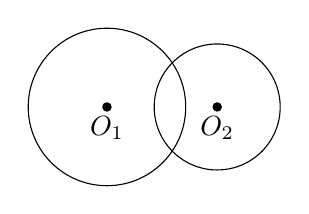
\begin{tikzpicture}
    \draw (0,0) circle (1);
    \draw (1.4,0) circle (.8);
    \node at (0,0)[below]{$O_1$};
    \node at (1.4,0)[below]{$O_2$};
    \draw (0,0)[fill=black] circle (1.5pt);
    \draw (1.4,0)[fill=black] circle (1.5pt);
\end{tikzpicture}    
    \caption{}
\end{figure}

设$A=\{X|X\text{为$\odot O_1$内的点}\}$,$B=\{X|X\text{为$\odot O_2$内的点}\}$,$\alpha$表示$\odot O_1$内的点,$\beta$表示$\odot O_2$内的点。则$A,B$与$\alpha,\beta$的关系如下(图2.16):
\begin{itemize}
    \item $A\cap B \longleftrightarrow \alpha\wedge \beta$\quad 在$\odot O_1$且在$\odot O_2$内的点的集合。
    \item $A\cup B\longleftrightarrow \alpha\vee \beta$\quad 在$\odot O_1$或在$\odot O_2$内的点的集合。
    \item $A^c\longleftrightarrow \bar{\alpha}$\quad 不在$\odot O_1$内的点的集合。
    \item $B^c\longleftrightarrow \bar{\beta}$\quad 不在$\odot O_2$内的点的集合。
    \item $A^c\cap B^c\longleftrightarrow \bar\alpha\wedge\bar\beta $\quad 不在$\odot O_1$内且不在$\odot O_2$内的点的集合。
    \item $A^c\cup B^c\longleftrightarrow \bar\alpha\vee\bar\beta$\quad 不在$\odot O_1$内或不在$\odot O_2$内的点的集合。
\end{itemize}

总结以上讨论,我们把性质与集合之间的关系列成下表:
\begin{center}
    \begin{tabular}{cc|cc}
\hline
        集合  & 性质 &集合  &性质\\
\hline
$A$ & $\alpha$ & $B$ & $\beta$\\
$A^c$ & $\bar\alpha$ & $B^c$ & $\bar\beta$\\
$A\cap B$ & $\alpha\wedge \beta$ & $A\cup B$ & $\alpha\vee\beta$\\
$A\subseteq B$ & $\alpha\Rightarrow\beta $& $A=B$&$\alpha\Leftrightarrow \beta$\\
\multicolumn{2}{c|}{$A\subseteq B$与$B\subseteq A^c$同义}& \multicolumn{2}{|c}{$\alpha\Rightarrow\beta$与$\bar\beta\Rightarrow\bar\alpha$同义}\\
\hline
    \end{tabular}
\end{center}

\subsection{基本逻辑语句}
\subsubsection{命题}
凡可决定其真假的语句就叫做\textbf{命题}。例如:
\begin{enumerate}
    \item 雪是白的。(真)
    \item 对顶角相等。(真)
    \item $2+2=5$。 (假)
    \item 若$x>y$, 则$\frac{x+2y}{3}>\frac{x+y}{2}$。(假)
\end{enumerate}

这些语句都是命题。从上面这些命题中我们可以看到,命题不一定为数学所独有,如1就不是数学命题,另外我们还看到一个命题是可以判断真假的,有的容易判断如1、2、3。有的就较难判断一些,如4是个假命题,但一眼
不容易看出来,实际上如果设$x=1$, $y=0,\;(x>y)$那么
$\frac{1+2\x 0}{3}\not>\frac{1+0}{2}$。这就说明4是个假命题了。所谓“判断真假”是对事物的本质说的,并不要求现在就要,“决定”,也不要求最近的将来便可决定。例如:
\begin{itemize}
    \item 别的星球上有生物。
    \item 凡大于4的偶数都是两个奇质数之和(这就是著名的哥德巴赫猜想)。
\end{itemize}

这些语句的真假不但现在不能决定,在最近的将来也未必“可决定”,但是我们认为从事物的本质来说,它们本身是有真假可言的,所以应该承认它们都是命题。

数学命题,经常使用“如果……,那么……”,“若……,则……。”的叙述形式,如前面提到的4便是这一类形式的
命题。这类命题写成一般形式就是:
\begin{blk}{}
若$\alpha$, 则$\beta$\qquad 或\qquad  如果$\alpha$, 那么$\beta$.
\end{blk}

下面我们仔细的分析它的结构和逻辑关系。

命题“若$\alpha$, 则$\beta$”是否正确,就要看$\alpha$、$\beta$之间是否具有推出关系$\alpha\Rightarrow\beta$了。也就是说,如果$\alpha$、$\beta$之间具有$\alpha\Rightarrow\beta$的关系,则“若$\alpha$, 则$\beta$”是真命题(即正确的命题),由此可见“$\alpha\Rightarrow\beta$”与“若$\alpha$, 则$\beta$”是真命题是同一关系的两种不同说法。

在命题“若$\alpha$, 则$\beta$”中,我们把$\alpha$叫做命题的\textbf{条件},$\beta$叫做命题的\textbf{结论}。

把“若$\alpha$, 则$\beta$”中的$\beta$作为条件,$\alpha$作为结论,就得到另一个命题:若$\beta$, 则$\alpha$. 这个命题叫做“若$\alpha$, 则$\beta$”的\textbf{逆命题}。

把“若$\alpha$, 则$\beta$”中的$\alpha$的反性质:非$\alpha$, $\beta$的反性质:非$\beta$, 分别作为条件和结论,又得到一个新命题:若$\bar\alpha$, 则$\bar\beta$, 这个命题叫做“若$\alpha$, 则$\beta$”的\textbf{否命题}。

把“若$\alpha$, 则$\beta$”中的$\beta$的反性质:非$\beta$, $\alpha$的反性质:非$\alpha$, 分别作为条件和结论,又可得到一个新命题:若$\bar\beta$, 则$\bar\alpha$. 这个命题叫做“若$\alpha$, 则$\beta$”的\textbf{逆否命题}。

若“$\alpha$, 则$\beta$”则叫做上述逆命题,否命题、逆否命题的\textbf{原命题}。这就是说,逆命题,否命题,逆否命题都是对原命题而说的,在四种命题中任何一个命题都可作为原命题。如:
\begin{itemize}
    \item 原命题\quad 若$\bar\alpha$,则$\bar\beta$
    \item 逆命题\quad 若$\bar\beta$,则$\alpha$
    \item 否命题\quad 若$\alpha$,则$\beta$($\bar\alpha$的非是$\alpha$,$\bar\beta$的非是$\beta$)
    \item 逆否命题\quad 若$\beta$,则$\alpha$
\end{itemize}

我们把上述四种命题之间的关系,列成下图:
\begin{center}
\begin{tikzpicture}[>=latex]
\node (A)[draw, rectangle]at (-3,2) {原命题:若$\alpha$,则$\beta$}; 
\node (B)[draw, rectangle]at (3,2) {逆命题:若$\beta$,则$\alpha$}; 
\node (C)[draw, rectangle]at (-3,-2){否命题:若$\bar\alpha$,则$\bar\beta$}; 
\node (D)[draw, rectangle]at (3,-2) {逆否命题:若$\bar\beta$,则$\bar\alpha$}; 
\node (E)[draw, rectangle, rounded corners=3mm]at (0,0) {互为逆否}; 
\draw[<->, ultra thick](A)--node[above]{互逆}(B);
\draw[<->, ultra thick](C)--node[below]{互逆}(D);
\draw[<->, ultra thick](A)--node[left]{互否}(C);
\draw[<->, ultra thick](B)--node[right]{互否}(D);
\foreach \x in {A,B,C,D}
{
    \draw[->, ultra thick](E)--(\x);
}
\end{tikzpicture}
\end{center}

\begin{example}
    写出“对顶角相等”这个命题的逆命题,否命题和逆否命题。
\end{example}

\begin{solution}
“对顶角相等”这个命题是由两部分组成的:(1)两个角是对顶角,(2)这两个角相等。(1)是命题的条件,(2)是命题的结论。这个命题若用“若—则”连结(1)、(2)两部分,就可写成。

若两个角是对顶角,则这两个角相等。所以,
\begin{itemize}
    \item 逆命题\quad 若两个角相等,则这两个角是对顶角。
    \item 否命题\quad 若两个角不是对顶角,则这两个角就不相等。
    \item 逆否命题\quad 若两个角不相等,则这两个角就不是对顶角。
\end{itemize}
\end{solution}

从这个例子,我们会发现,在这四个命题中有的正确,有的不正确,那么,这四种命题的真假之间是否存在某种关系呢?下面我们再举两个例子。

\begin{example}
    写出“如果一个数末位数字是0,那么它一定能被5整除。”这个命题的逆命题,否命题、逆否命题。
\begin{itemize}
    \item 原命题\quad 如果一个数末位数字是0, 那么它一定能被5整除(真)。
    \item 逆命题\quad 如果一个数能被5整除,那么它的末位数字一定是0(假)。
    \item 否命题\quad 如果一个数末位数字不是0, 那么它一定 不能被5整除(假)。
    \item 逆否命题\quad 如果一个数不能被5整除,那么它的末位数字一定不是0(真)。
\end{itemize}
\end{example}

\begin{example}
    写出“若某人是中国人,则他是北京人。”这个命题的逆命题、否命题、逆否命题。

\begin{itemize}
    \item 原命题\quad 若某人是中国人,则他是北京人(假)。
    \item 逆命题\quad 若某人是北京人,则他是中国人(真)。
    \item 否命题\quad 若某人不是中国人,则他不是北京人(真)。
    \item 逆否命题\quad 若某人不是北京人,则他不是中国人(假)。
\end{itemize}
\end{example}

从以上的例子,我们看到原命题和逆否命题同真假,逆命题和否命题同真假。










